\chapter{Explorations in games on networks}\label{ch:games-on-networks}
\section{Game theory}
\subsection{Prisoner's Dilemma}\label{subs:prisoners-dilemma}
The Prisoner's Dilemma is the canonical game of game theory finding its use in models for everything from how firms price goods\cite{p-d-goods} to sharing in vampire bats\cite{p-d-nature}. In any situation where there is the possibility of cooperation, the Prisoner's Dilemma can be a useful model in understanding the situation to a first approximation.\\
\\
%\paragraph{The Story}
The motivating story goes that two accomplices are caught at a crime scene, arrested and placed in separate cells with no contact. The police give them each a choice: they can confess their crimes to the authorities or they can stay silent. They learn that if they both stay silent, they only get one year in prison. If they both confess, they both get two years. However, if one of them confesses and the other stays silent, the snitch gets out immediately while the snitched-upon gets 3 years. As they are in separate cells, they cannot communicate.\\
\\
The smallest combined time in prison for the couple is if they both stay silent and take 1 year in jail each. But even if they could communicate and agree to the appealing option of both staying silent, it would still make sense to defect from the `contract' and confess. Just 1 year in jail is clearly better than 2. How should they work through this? As with most things in life, they should get mathematical.
\subsubsection{Making this mathematical}
%\paragraph{Key Concepts}
This story has all the features of a game-theoretic game. Let's go through it, pick out the key elements and name them.\\
\\
The four essential elements of a game have a useful acronym: \textit{PAPI}\cite{rasmusen_2010}. This stands for:
\begin{enumerate}[nosep]
\item \textbf{P}layers of the game,
\item \textbf{A}ctions available to each player,
\item \textbf{P}ayoffs for each outcome
\item \textbf{I}nformation available to each player.
\end{enumerate}
\par\null\par
In our story, there are two players: Lou and Avery. There are two actions available to them: stay silent or confess.  The payoffs are given by the years in jail, $-x$ for $x$ years in jail. As they cannot communicate, there is no information available about the other player's choice prior to choosing.\\
\\
Formally, we call staying silent a decision to \textit{cooperate} with the partner. We also say that to confess is to \textit{defect} from their partner. We usually notate actions as a single letter. Here we write $C$ for cooperate and $D$ for defect. An \textit{outcome} defines an action for each player. It can be written $(C,C)$ for two players both playing the action $C$.\\
\\
%\subsubsection{Representing games}
%\subsubsection{Payoff Matrix}
A payoff matrix is a way of defining two-player simultaneous games completely\cite{osborne}. This means that it tells you about every element of \textit{PAPI}. The payoff matrix for the Prisoner's Dilemma given in the story would be:\\
\setlength{\extrarowheight}{2pt}
\begin{tabular}{cc|c|c|}
	\centering
	& \multicolumn{1}{c}{} & \multicolumn{2}{c}{Avery}\\
	& \multicolumn{1}{c}{} & \multicolumn{1}{c}{$C$}  & \multicolumn{1}{c}{$D$} \\\cline{3-4}
	\multirow{2}*{Lou}  & $C$ & $(-1,-1)$ & $(-3,0)$ \\\cline{3-4}
	& $D$ & $(0,-3)$ & $(-2,-2)$ \\\cline{3-4}
\end{tabular}
\\
\\
\\
The ordered pair $(x,y)$ in each matrix entry gives the payoffs for each outcome. $x$ gives the payoff for the horizontal player and $y$ gives the vertical player's. So outcome $(D,C)$ has payoff $(0,-3)$ meaning a payoff of $0$ for Lou for defecting and a payoff of $-3$ for Avery for cooperating. The players, actions and payoffs are defined. Also, in a simultaneous game there is no information available about the other player's action. So this matrix does indeed completely describe the game.\\
\\
The payoff matrix is an extremely useful representation, allowing concise, complete descriptions of games. Consider, for example:\\
\setlength{\extrarowheight}{2pt}
\begin{tabular}{cc|c|c|c|}
	& \multicolumn{1}{c}{} & \multicolumn{3}{c}{Avery} \\
	& \multicolumn{1}{c}{} & \multicolumn{1}{c}{$R$}  & \multicolumn{1}{c}{$P$}  & \multicolumn{1}{c}{$S$} \\\cline{3-5}
	& $R$ & $(0,0)$ & $(-1,1)$ & $(1,-1)$ \\ \cline{3-5}
	Lou  & $P$ & $(1,-1)$ & $(0,0)$ & $(-1,1)$ \\\cline{3-5}
	& $S$ & $(-1,1)$ & $(1,-1)$ & $(0,0)$ \\\cline{3-5}
\end{tabular}
\\
\\
\\
This game might initially look foreign, but it is simply Rock, Paper, Scissors. You can create stories to motivate them but the payoff matrix completely defines all the relevant mathematical aspects of the game. This allows us to abstract from the messy details of the human world and find `solutions' to the game.
\subsubsection{Strategies and solution concepts}
A \textit{strategy} is a set of rules that determine which action a player will use at each point of the game. Note that as the Prisoner's Dilemma has only one point to make a decision, a strategy determines just one action. Further a strategy profile determines a strategy for each player in the game. There are various ways to discuss the effectiveness of strategies and strategy profiles in a game.\\
\\
%\subsubsection{Strategies}
%\paragraph{Socially Optimal Strategy}
The \textit{socially optimal strategy profile} is the strategy profile that leads to the highest joint payoff for all players. That is, the sum of the payoffs is the highest of all possibilities. In this game this is the easily identifiable and clearly optimal option of both players cooperating so that they get only 1 year each.\\
\\
%\paragraph{Nash Equilibrium}
However, the outcome with both defecting is the \textit{Nash Equilibrium}. Informally, the Nash Equilibrium is an outcome in which, even if all players knew almost telepathically what the other player's actions were going to be, none of them would choose to change their action as it would not improve their payoff. In this game, both players defecting, $(D,D)$, is the unique Nash Equilibrium. This is because if one player, say Lou, knew that Avery would play $D$ he would not change to $C$. Similarly for Avery.\\
\\
%\paragraph{Dominant Strategy}
The outcome of $(D, D)$ actually satisfies an even stronger condition as the action $D$ is a \textit{dominant strategy} for both players. This means that no matter what action the opponent plays, the player will always get the best payoff by defecting. This is how $(D,D)$ manages to `pull' players in, despite it having a worse payoff for both players than $(C,C)$.\\
\\
So we have described three solution concepts. Which one do we predict will happen? Game theory assumes that players are \textit{rational}. This means that the payoffs match the player's desires and they desire to increase their payoff. In other words the payoffs accurately describe their preferences. If Lou and Avery are rational, they will always end up both defecting, betraying each other and being rewarded with a longer jail term. So it goes.
\subsection{Repeated games}\label{subs:repeated-games}
%\subsubsection{Introduction}
The Prisoner's Dilemma is a \textit{one-shot game}. This means that no further games are played after the first game. It happens once and never again, with no possible repercussions that are not already described in the payoff matrix.\\
\\
Unlike one-shot games, repeated games have players play multiple games against each other. Whereas before a strategy determined just one action, in a repeated game a strategy can respond to the other player's actions. This means that it is harder or even impossible to `solve' these games to find the best actions and equilibria. However, this makes them more interesting, allowing for complex dynamics.
\subsubsection{Iterated Prisoner's Dilemma}
If we have two players playing the Prisoner's Dilemma repeatedly against each other we create the Iterated Prisoner's Dilemma. This no longer has a best strategy.\\
\\
In the absence of an analytically provable `best' strategy, we can pursue a more empirical approach. In football we cannot prove a-priori the best team. Indeed it would be a bit boring if we could. Instead, we create a tournament such as the Premier League and declare the winner of the tournament the `best' team. Inspired by this approach, we create a `tournament' of different strategies all playing several hundred games of the Prisoner's Dilemma against each other. The winner of the tournament will be the strategy with the highest payoff overall.\\
\\
This numerical experiment was famously first done by Robert Axelrod\cite{axelrod} in the 1980s. In Axelrod's first tournament, the winner was `Tit for Tat', a strategy that always cooperates on the first round and then copies the opponent's previous move forever after. Since then other researchers have repeated the tournament and Axelrod himself ran a second tournament with many more entries. A recent open-source collaboration makes it easy to replicate the Axelrod's original tournament as well as run similar ones\cite{axelrod-github}.\\
\\
For the tournament, we choose to enter five strategies: Tit for Tat, Defector, Cooperator, Alternator and Random. The names are descriptive: Defector always defects, Cooperator always cooperates, Alternator alternates between the two and Random chooses between the two actions with probability $0.5$ at each point. They play against every other strategy $10$ times. They also play against themselves $10$ times. The payoffs are also altered to fit Axelrod's first tournament. They are given by $1$ for two defectors, $3$ for two cooperators and $5$ and $0$ for the defector and cooperator respectively.\\
\setlength{\extrarowheight}{2pt}
\begin{tabular}{cc|c|c|}
	& \multicolumn{1}{c}{} & \multicolumn{2}{c}{Avery}\\
	& \multicolumn{1}{c}{} & \multicolumn{1}{c}{$C$}  & \multicolumn{1}{c}{$D$} \\\cline{3-4}
	\multirow{2}*{Lou}  & $C$ & $(3,3)$ & $(0,5)$ \\\cline{3-4}
	& $D$ & $(5,0)$ & $(1,1)$ \\\cline{3-4}
\end{tabular}
\label{mmd}
\\
\\
Running the tournament reveals that `Defector' does best in this tournament (Fig. \ref{fig:iterated-p-d-tournament}). The key point is that there is no single strategy that dominates all the others. Whilst `Defector' does best in this tournament, with a different selection of strategies it probably would not. Indeed it was entered into Axelrod's first tournament and was beaten by Tit for Tat, a strategy it won against here. Whilst this may seem paradoxical it is no more paradoxical than a polar bear being better suited to Antarctica than a tiger but would struggle in Bali. That is, the strategies success is dependent on its environment. In it's extreme, a defector does well in a tournament full of unquestioning cooperators. However, in a tournament full of Tit For Tat strategies, the Tit for Tat strategies get consistently high payoffs through cooperation which the defector misses out on, instead getting the spoils of mutual defection.\label{mmd}
%\textit{Mark: This seems paradoxical - what is it about the tournament design that makes this possible?}
\begin{figure}
	\centering
	\begin{subfigure}{\textwidth}
		\centering
		\includegraphics[width=\linewidth]{axelrod/tournament-boxplot.png}
		\caption{The results of a tournament of the Prisoner's Dilemma between 5 strategies. The tournament was repeated 100 times. Due to the strategy `Random' the results were different each time. The plot shows the average payoff between all tournaments in the solid blue line and the shaded blue region represents the variance.
%		\textit{Mark: I don't understand this figure}
		\label{mmd}
		}
		\label{}
	\end{subfigure}%
\\
	\begin{subfigure}{\textwidth}
		\centering
		\includegraphics[width=0.95\linewidth]{axelrod/tournament-payoff-matrix.png}
		\caption{A payoff matrix showing how each strategy performed on average against the other strategies. The colour of the point $(X,Y)$ represents the score of strategy $X$ playing against strategy $Y$.}
		\label{}
	\end{subfigure}
	\caption{A tournament of the Iterated Prisoner's Dilemma between five strategies.}
	\label{fig:iterated-p-d-tournament}
\end{figure}\\
\\
We can create a grand competition with 222 different strategies. The strategies comprise every entry from a library of distinct strategies submitted to the Axelrod-Python project team\cite{axelrod-github}.\label{mmd} On this run the joint winners were: `Hard Prober', `Pun1' and `Tester'. For example Hard Prober's strategy is to play $D,D,C,C$ initially. This is to act as a test to see how cooperative its opponent is. If the opponent cooperated in moves 2 and 3, Hard Prober will defect forever. Otherwise, it will play Tit-For-Tat for the rest of time. The results of the tournament are messy to see as a plot, payoff matrix or indeed a table of the raw data. However, the alphabetically first 5 strategies are shown in Fig. \ref{fig:222}.
%\begin{tabular}{1|1}
%	\csvreader[head to column names]{images/csv/axelrod-tournament-222.csv}{}
%	{\\\hline\csvcoli&\csvcolii}
%\end{tabular}
\begin{figure}
\csvautotabular{../data/axelrod-tournament-222-short.csv}
\caption{A table of the alphabetically first 5 strategies in an iterated Prisoners Dilemma tournament of 222 different strategies.}
\label{fig:222}
\end{figure}
\subsubsection{Iterated games with evolution}
One natural extension to iterated games is to allow the possibility of `evolutionary' behaviour. For example, we can create simulations where strategies with higher payoffs are more likely to produce `offspring'. This means that the number of players using a successful strategy tends to increase.\\
\\
This can be imagined in the ordinary evolutionary sense of survival of the fittest. However, there is another useful interpretation. We can view the population as a constant group of players who are open to the possibility of changing their strategies. If they see a strategy that is working better, there is some probability that they use that strategy in the next iteration.\\
\\
We randomly select $7$ players using strategies from Axelrod's tournament. We play them off each other and themselves. After each round, they have some chance of `reproducing' proportional to the payoff they just received from playing every other player. Then the next round has a population that tends to have more of the successful strategies and less of the poorly adapted strategies. A graph describing this is given in Fig. \ref{fig:moran-100}.
\begin{figure}
	\centering
	\includegraphics[width=\linewidth,trim={0 0 0 2cm},clip]{axelrod/iterated-moran-7.png}
	\caption{A graph showing an evolutionary prisoner's dilemma tournament.\label{mmd}. At each iteration or tick one agent is chosen to reproduce and one agent is chosen to die. The probability that they are chosen to reproduce is proportional to their payoff in the previous round.}
	\label{fig:moran-100}
\end{figure}
\\
\\
%[Include replicator equations at some point here.]\\
%For example, we can also try it with different gamesbelow is a simulation of strategies playing Rock, Paper Scissors defined by the payoff matrix as above.\\
%(
%My simulation of Rock, Paper, Scissors
%)\\
%The effect is a self-balancing system. If the strategy \textit{rock} becomes more populous, \textit{paper} will start to get higher payoffs on average. This in turn brings the population back towards $\frac{1}{3}$ for each strategy.\\
%The same scenario works with the admittedly less well-known game Rock, Paper, Scissors, Spock\cite{for game}\cite{for code}.\\
%(
%My simulation of Rock, Paper Scissors, Spock
%)\\
%However, now with the different rules we can have the extinction of strategies.
We can explore the same evolutionary set-up but with the game of Rock, Paper, Scissors. Whereas evolutionary Prisoner's Dilemma resulted in one strategy eventually monopolising the population, the evolution of Rock, Paper, Scissors results in a self-balancing system (Fig. \ref{rock-paper-scissors-evo}). For example if the strategy Rock becomes more populous, Paper will start to get higher payoffs on average. This gives Paper a higher chance of reproducing resulting in Paper reproducing at a quicker rate. This holds for all three pairs. So the population has an inbuilt tendency to return the population demographic back towards $\frac{1}{3}$ for each strategy.\label{mmd}
\begin{figure}
	\centering
	\includegraphics[width=\linewidth]{axelrod/rock-paper-scissors.png}
	\caption{An evolutionary game of Rock, Paper, Scissors. The graph shows the percentage of players changing through time.}
	\label{rock-paper-scissors-evo}
\end{figure}
\section{Graph theory}\label{sec:graph-theory}
%motivation
The tools we have built so far are helping us move closer to a reasonable description of real, complex situations. In real life, games are not usually isolated situations that happen as if in a laboratory. They happen around lots of other players and allow the possibility of a change of strategy. They are also interdependent with games in some places effecting others. If a person was playing the Prisoner's Dilemma and played against several defectors consecutively, they are more likely to defect themselves. We have begun to model this.\\
\\
However, players are in general not connected to every other player. They exist in communities. To model this we need graphs.\\
\\
\subsection{Definitions}
A \textit{graph} $G=(V,E)$ is a set of vertices $V$ and a set of pairs of vertices $E$. Each pair of vertices is called an edge. For now we will consider only undirected graphs with no loops . \textit{Undirected} means that the edge $(u,v)$ is identical to the edge $(v,u)$. That is to say, the pairs constituting the edges are unordered\cite{graph-theory-reference}. The requirement of no loops means that no vertex has an edge from itself to itself. Formally, $\nexists v\textnormal{ such that } (v,v)\in E$. We can see visually what this means in Fig. \ref{fig:example-graphs}.
\begin{figure}
	\centering
	\begin{subfigure}{.3\textwidth}
		\centering
		\includegraphics[width=.9\linewidth]{appendix/graph-theory/directedGraph.png}
		\caption{Directed graph}
		\label{fig:dir}
	\end{subfigure}%
	\begin{subfigure}{.3\textwidth}
		\centering
		\includegraphics[width=.9\linewidth]{appendix/graph-theory/loopGraph.png}
		\caption{Graph with loops}
		\label{fig:loop}
	\end{subfigure}
	\begin{subfigure}{.3\textwidth}
		\centering
		\includegraphics[width=.9\linewidth]{appendix/graph-theory/graph.png}
		\caption{Undirected graph without loops}
		\label{fig:undirected}
	\end{subfigure}
	\caption{We will consider graphs of type \ref{fig:undirected} and ignore the others.}
	\label{fig:example-graphs}
\end{figure}
\\
\\
Two vertices $u,v$ are \textit{adjacent} if and only if $(u,v)\in E$. The neighbourhood of a vertex $v$ in a graph $G$ is the induced graph given by $v$ and all vertices adjacent to $v$. That is, it is the graph of vertex $v$ and all vertices adjacent to $v$ with edges given by the edges between any of these vertices in $G$. As such we also call the adjacent vertices \textit{neighbours}.\\
\\
%Some common graphs
A useful graph that comes up repeatedly is the \textit{complete graph, $K_n$}. This is the graph with $n$ vertices with an edge between all pairs of vertices. Formally $K_n=\{\{v_1,...,v_n\},\{(v_i,v_j):\forall i\neq j\}\}$.
\begin{figure}
	\centering
	\begin{subfigure}{.5\textwidth}
		\centering
		\includegraphics[width=.9\linewidth]{appendix/games-on-networks/K5.pdf}
		\caption{$K_5$}
		\label{fig:K5}
	\end{subfigure}%
	\begin{subfigure}{.5\textwidth}
		\centering
		\includegraphics[width=.9\linewidth]{appendix/games-on-networks/K16.pdf}
		\caption{$K_{16}$}
		\label{fig:K16}
	\end{subfigure}
	\caption{The Complete Graphs $K_5$ and $K_{16}$}
	\label{fig:complete-graphs}
\end{figure}
\subsection{Graphs and the 2D lattice}
A graph often used in models is an adaptation of the 2D lattice as it is both instructive, relatively easy to analyse and most importantly easy to visualise\cite{eq_of_life}. The 2D lattice can be made by imagining a square grid, rows and columns of squares.
%\begin{figure}
%	\centering
%	\includegraphics[width=.5\linewidth]{appendix/graph-theory/square-grid.png}
%	\caption{A square grid}
%\end{figure}
However, we want to convert this into a graph. We can deal with the vertices easily: we put a vertex at the centre of each square. However there are multiple ways to define the edges. Which squares should be considered neighbours of each other?\\
\\
One option is to define the von Neumann neighbourhood of the 2D lattice as in Fig. \ref{fig:vonneumann}. This makes each point a neighbour of the $4$ points vertically and horizontally next to it. An alternative is given by the Moore neighbourhood as seen in Fig. \ref{fig:moore}. This includes the nearest vertical and horizontal neighbours as well as the nearest diagonal points\cite{eq_of_life}.
\begin{figure}
	\centering
	\begin{subfigure}{.5\textwidth}
		\centering
		\includegraphics[width=.9\linewidth]{appendix/graph-theory/von-neumann-neighbourhood.png}
		\caption{The von Neumann Neighbourhood}
		\label{fig:vonneumann}
	\end{subfigure}%
	\begin{subfigure}{.5\textwidth}
		\centering
		\includegraphics[width=.9\linewidth]{appendix/graph-theory/moore-neighbourhood.png}
		\caption{The Moore neighbourhood}
		\label{fig:moore}
	\end{subfigure}
	\caption{Different definitions of `neighbourhood' on the 2D Lattice}
	\label{fig: lattice neighbourhoods}
\end{figure}\\
\\
The graphs given by these two definitions are given in Fig. \ref{fig:graph-neighbourhoods}. The graph induced by the von Neumann neighbourhood is often called the grid graph, lattice graph. The graph induced by the Moore neighbourhood is also called the King's Graph as it represents the legal moves of a king in a game of chess.
\begin{figure}
	\centering
	\begin{subfigure}{.47\textwidth}
		\centering
		\includegraphics[width=\linewidth]{appendix/graph-theory/grid-graph.png}
		\caption{}
		\label{fig:graph-v-n}
	\end{subfigure}
	\begin{subfigure}{.47\textwidth}
		\centering
		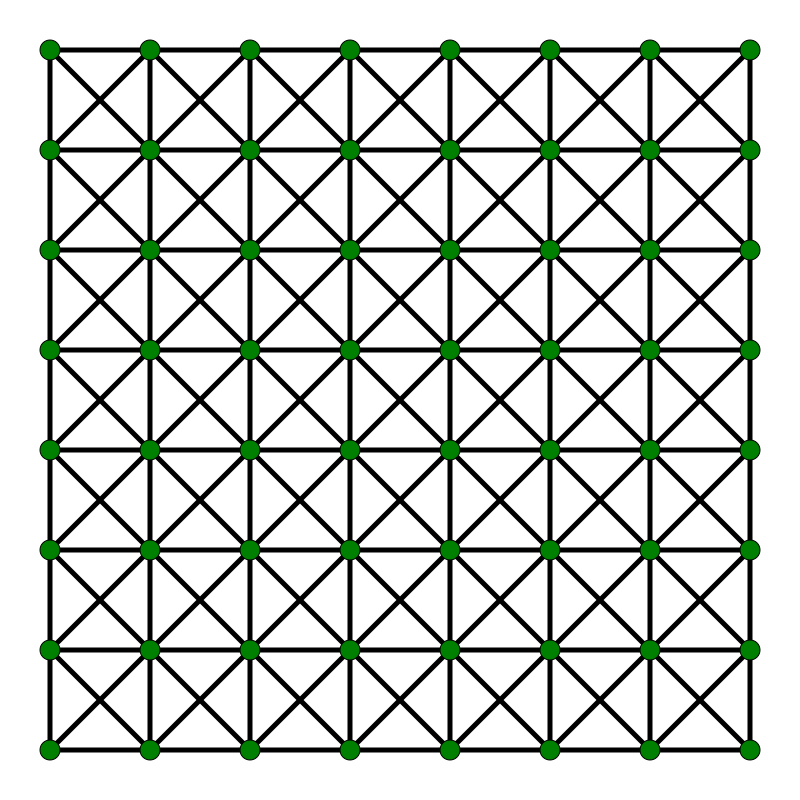
\includegraphics[width=\linewidth]{appendix/graph-theory/kings-graph.png}
		\caption{}
		\label{fig:graph-m}
	\end{subfigure}
	\caption{Graph representation of the 2D lattice with the von Neumann neighbourhood\ref{fig:graph-v-n} and the Moore neighbourhood \ref{fig:graph-m}}
	\label{fig:graph-neighbourhoods}
\end{figure}\\
\\
Typically to avoid boundary effects when playing games on these lattices we `wrap' the 2D lattice. This creates a torus. So each vertex displayed visually at the top of the lattice is joined to the neighbour in the same column at the bottom of the lattice. This avoids, for example, the side players having fewer opponents. However it makes it harder to visualise explicitly and so is normally drawn in two-dimensions with no visual representation of the wrapping.
\section{Games on networks}
%\subsubsection{Games on graphs we have already seen}
Having further built up our tool-kit, we can now consider games on graphs. We set each vertex to represent a player and only allow players to play a game against players they are adjacent to. In fact, we have sneakily been doing this the whole time but now we want to make this explicit.\\
\\
The basic Prisoner's Dilemma in \ref{subs:prisoners-dilemma} was a game on a trivial graph $G=(\{Lou,Avery\},\{(Lou,Avery)\})$, visualised in Fig. \ref{fig:p-d-graph}.
\begin{figure}[h]
	\centering
	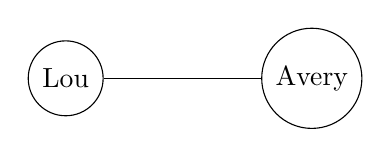
\begin{tikzpicture}
	\draw
	(1,1) node[anchor=east,circle,draw]{Lou}--
	(3,1) node[anchor=west,circle,draw]{Avery};
	\end{tikzpicture}
	\caption{The trivial graph underlying the one-shot Prisoner's Dilemma}
	\label{fig:p-d-graph}
\end{figure}
Similarly, for the Iterated Prisoner's dilemma tournament if we call the players $p_1,...,p_n$, the tournament was a repeated game on a complete graph $K_n$.\\
\\
%\subsubsection{Some new Graphs}
So we were already playing games on graphs implicitly. Now we can try building games while noting the graphs we are playing on explicitly and seeing what effect this has.
\subsection{Prisoner's Dilemma on a torus}\label{p-d-torus}
%\subsubsection{Set-up}
We can extend the Iterated Prisoner's Dilemma to a tournament on a 2D lattice. Firstly, we make an $n \times n$ grid with wrapped ends to avoid boundary effects, creating a torus. Using the process seen in the previous section we make a graph out of this using the Moore neighbourhood. Then we let each vertex be a player of the Prisoner's Dilemma. They play against all other vertices in their neighbourhood\cite{eq_of_life}.\\
\\
To initialise the system, in the first round each player plays $C$ with probability $p$ and $D$ with probability $(1-p)$. They play this action simultaneously against every neighbour, using the same strategy against each of them.\\
\\
For every round after, each player looks at their neighbour's scores from the previous round. They adopt the action of the highest scoring neighbour as their action for the next round\footnote{For most parameter values chosen, ties are only possible between cells that use the same strategies and so this is well-defined. If there were to be a tie between two distinct strategies, the strategy adopted would arbitrarily be the strategy closest to the top left of the grid.}\label{mmd} They then play this action against every neighbour.\\
\\
The payoff matrix retains characteristics of the matrix originally given for the Prisoner's Dilemma and is given by:\\
\setlength{\extrarowheight}{2pt}
\begin{tabular}{cc|c|c|}
	& \multicolumn{1}{c}{} & \multicolumn{2}{c}{Avery}\\
	& \multicolumn{1}{c}{} & \multicolumn{1}{c}{$C$}  & \multicolumn{1}{c}{$D$} \\\cline{3-4}
	\multirow{2}*{Lou}  & $C$ & $(1,1)$ & $(\epsilon,b)$ \\\cline{3-4}
	& $D$ & $(b,\epsilon)$ & $(0,0)$ \\\cline{3-4}
\end{tabular}
\\
\\
where $\epsilon<1<b$.\\
\\
%\subsubsection{Example Runs}
To run this we simulate on a $100\times100$ grid and choose values $p=0.5$ and $\epsilon=0$. We can create a wide variety of dynamic behaviour, including chaos and bifurcations by adjusting the value of $b$. Note that $b$ is the payoff from defecting against a cooperative partner. Intuitively, it is the reward to true villains who defect against players who were hoping to cooperate.
\subsubsection{Qualitative analysis: equilibrium and chaos}
For $b>1.\bar{6}$, the board eventually tends to an equilibrium with mostly defectors (Fig. \ref{fig:p-d-torus-1.7}). Clearly the rewards of non-cooperation are too high to a sustain a more socially beneficial situation.
\begin{figure}
	\centering
	\begin{subfigure}{.3\textwidth}
		\centering
		\includegraphics[width=.9\linewidth]{appendix/games-on-networks/pd-torus/1b=17.png}
		\caption{Early}
		\label{}
	\end{subfigure}%
%	\begin{subfigure}{.3\textwidth}
%		\centering
%		\includegraphics[width=.9\linewidth]{appendix/games-on-networks/pd-torus/2b=17.png}
%		\caption{Developing}
%		\label{}
%	\end{subfigure}
	\begin{subfigure}{.3\textwidth}
		\centering
		\includegraphics[width=.9\linewidth]{/appendix/games-on-networks/pd-torus/3b=17.png}
		\caption{Equilibrium}
		\label{}
	\end{subfigure}
	\caption{The simulation running with $b=1.7$}
	\label{fig:p-d-torus-1.7}
\end{figure}
Conversely, for $b<1.6$, the simulation tends towards a static equilibrium of mainly cooperators (Fig. \ref{fig:p-d-torus-1.5}).
\begin{figure}
	\centering
	\begin{subfigure}{.3\textwidth}
		\centering
		\includegraphics[width=.9\linewidth]{appendix/games-on-networks/pd-torus/1b=15.png}
		\caption{Early}
		\label{fig:dir}
	\end{subfigure}%
	\begin{subfigure}{.3\textwidth}
		\centering
		\includegraphics[width=.9\linewidth]{appendix/games-on-networks/pd-torus/2b=15.png}
		\caption{Developing}
		\label{fig:loop}
	\end{subfigure}
	\begin{subfigure}{.3\textwidth}
		\centering
		\includegraphics[width=.9\linewidth]{appendix/games-on-networks/pd-torus/3b=15.png}
		\caption{Equilibrium}
		\label{fig:undirected}
	\end{subfigure}
	\caption{The simulation running with $b=1.5$}
	\label{fig:p-d-torus-1.5}
\end{figure}
Between these two parameter regions, exists the third which exhibits the most interesting behaviour with chaotic dynamics between cooperation and defection (Fig. \ref{fig:p-d-torus-1.63}).
\begin{figure}
	\centering
	\begin{subfigure}{.3\textwidth}
		\centering
		\includegraphics[width=.9\linewidth]{appendix/games-on-networks/pd-torus/1b=163.png}
		\caption{Early}
		\label{fig:dir}
	\end{subfigure}%
	\begin{subfigure}{.3\textwidth}
		\centering
		\includegraphics[width=.9\linewidth]{appendix/games-on-networks/pd-torus/2b=163.png}
		\caption{Developing}
		\label{fig:loop}
	\end{subfigure}
	\begin{subfigure}{.3\textwidth}
		\centering
		\includegraphics[width=.9\linewidth]{appendix/games-on-networks/pd-torus/3b=163.png}
		\caption{Dynamic equilibrium}
		\label{fig:undirected}
	\end{subfigure}
	\caption{The simulation running with $b=1.63$}
	\label{fig:p-d-torus-1.63}
\end{figure}
\subsubsection{Quantitative analysis: invasion}
The usual approach for understanding evolutionary games is to find the conditions under which one type can `invade' a population. An invasion is when a small group of one type can grow in a population of other types. To do this with our game we must analyse the situation from the level of individual squares.\\
\\
Firstly, we need to find the minimal area that we can isolate to study. A single cell plays against it's surrounding neighbours and so we must consider at least the $3\times3$ grid surrounding a cell. However, the cell then adopts the strategy of all of its best performing neighbours. So it must look at its neighbour's payoffs. But it's neighbours payoffs depend on the games \textit{they} have just played against \textit{their} neighbours. So, to know what strategy our single cell will adopt we have to consider the surrounding $5\times5$ grid\cite{eq_of_life}.\\
\\
We will call the small population of potential invaders the \textit{cluster} and the rest of the population the \textit{sea}. Then we call the cells that are in the sea touching the cluster the \textit{boundary}. The general strategy we have will be to look at the boundary separating the small cluster of invaders from the rest of the population. If the boundary cells have a neighbour in the cluster with a better tactic than their neighbours in the sea, they will change and the cluster will grow.\\
\\
Let's first consider the conditions under which defectors can invade cooperators. Imagine a single defector in a sea of cooperators (Fig. (\ref{fig:1-d-i})). After the first game, the defector gets a payoff of $8b$, the boundary cells all get $7$ while all members of the sea get $8$. So the boundary members look to see if $8b>8$. As the game specifies that $b>1$, this is always true and so regardless of the value of $b$ it grows to a $3\times3$ grid.
\begin{figure}
	\centering
	\begin{subfigure}{.49\textwidth}
		\centering
		\includegraphics[width=.9\linewidth]{appendix/games-on-networks/pd-torus/1-defector-invasion.png}
		\caption{1 defector invasion}
		\label{fig:1-d-i}
	\end{subfigure}%
	\begin{subfigure}{.49\textwidth}
		\centering
		\includegraphics[width=.9\linewidth]{appendix/games-on-networks/pd-torus/9-defector-invasion.png}
		\caption{9 defector invasion}
		\label{fig:9-d-i}
	\end{subfigure}
	\caption{Defector invasion}
	\label{}
\end{figure}\\
\\
So now we consider a $3\times3$ grid of defectors (Fig. (\ref{fig:9-d-i})). The sea cells always have a higher payoff ($8$) than the boundary (either $5,6$ or $7$). The highest scoring cell in the cluster is the edge cell with a payoff of $5b$. Every cell of the boundary is a neighbour to an edge cell. Hence each cell looks to see if $5b>8$. If it is, they change and the cluster grows. Otherwise, it stays the same or shrinks. So to have the possibility of defector invasion we need $b>8/5=1.\dot6$.\\
\\
Now we consider cooperator invasion. We firstly note that a single cooperator cannot invade a population due to the constraints on the payoff matrix (Fig. (\ref{fig:1-c-i})). The defectors can simply feed off the foolishness of the sole cooperator and it will die off. Hence a cooperator invasion must start with some cluster.
\begin{figure}
	\centering
	\begin{subfigure}{.3\textwidth}
		\centering
		\includegraphics[width=.9\linewidth]{appendix/games-on-networks/pd-torus/1-cooperator-invasion.png}
		\caption{1 cooperator invasion}
		\label{fig:1-c-i}
	\end{subfigure}%
	\begin{subfigure}{.3\textwidth}
		\centering
		\includegraphics[width=.9\linewidth]{appendix/games-on-networks/pd-torus/4-cooperator-invasion.png}
		\caption{4 cooperator invasion}
		\label{fig:4-c-i}
	\end{subfigure}
	\begin{subfigure}{.3\textwidth}
		\centering
		\includegraphics[width=.9\linewidth]{appendix/games-on-networks/pd-torus/9-cooperator-invasion.png}
		\caption{9 cooperator invasion}
		\label{fig:9-c-i}
	\end{subfigure}
	\caption{Cooperator invasions}
	\label{}
\end{figure}
\\
\\
Looking at a $2\times2$ cluster of cooperators (Fig. (\ref{fig:4-c-i})), it is easy to see that if $b>3/2$ the cluster will grow uniformly. Otherwise it will be immediately destroyed.\\
\\
With a $3\times3$ cluster of cooperators there are different possibilities for growth (Fig. (\ref{fig:9-c-i})). Cell $A$ looks at the payoff of cell $B$ which is $2b$ against the payoff of it's only cluster neighbour which has a payoff of $3$. So if $3>2b$ it will change. If this is the case $B$ and $C$ will also both change.\\
\\
However, if $b>3/2$ there is still the possibility of $B$ and $C$ changing whilst $A$ stays the same. The highest scoring neighbour of cells $B,C$ will be either $C$ with payoff $3b$ or the cluster cell with payoff $5$. So they look to see if $5>3b$. If so they will change and the cluster will grow. This will create a cross structure.
\begin{figure}[h]
	\centering
	\caption{The payoffs of cells around a $3\times3$ cluster of cooperators in a sea of defectors.}
	\label{fig:p-d-graph}
\end{figure}
To summarise defector clusters can grow if $b>8/5=1.6$ and cooperator clusters can grow if $1.\dot6=5/3>b$. So there are three distinct parameter regions
\begin{enumerate}
	\item $b<1.6$ Only cooperator clusters can grow
	\item $1.6<b<1.\dot6$ Both cooperator and defector clusters can grow\label{chaos}
	\item $1.\dot 6<b$ Only defector clusters can grow
\end{enumerate}
This analytical approach justifies the conclusions we drew qualitatively earlier. In particular, region \ref{chaos}., where both defectors and cooperators can grow, represents the chaotic region.
%\subsubsection{Prisoner's Dilemma on a Scale Free Graph}
%\subsubsection{On Different Networks}
%We can adapt this to a hexagonal lattice.
%\begin{figure}
%	\centering
%	\begin{subfigure}{.3\textwidth}
%		\centering
%		\includegraphics[width=.9\linewidth]{appendix/games-on-networks/pd-hexagon/0005.png}
%		\caption{}
%		\label{fig:dir}
%	\end{subfigure}%
%	\begin{subfigure}{.3\textwidth}
%		\centering
%		\includegraphics[width=.9\linewidth]{appendix/games-on-networks/pd-hexagon/0012.png}
%		\caption{}
%		\label{fig:loop}
%	\end{subfigure}
%	\caption{Running the evolutionary Prisoner's Dilemma on a hexagonal lattice}
%	\label{fig:p-d-torus-1.63}
%\end{figure}